% !TeX root = ../main-english.tex
% !TeX spellcheck = en-US
% !TeX encoding = utf8
% -*- coding:utf-8 mod:LaTeX -*-

%This smart spell only works if no changes have been made to the chapter
%using the options proposed in preambel/chapterheads.tex.
\setchapterpreamble[u]{%
	\dictum[Ian Holmes, in an \href{https://twitter.com/ianholmes/status/288689712636493824}{\#overlyhonestmethods tweet}]{You can download our code from the URL supplied. Good luck downloading the only	postdoc who can get it to run, though.}
}


\chapter{Ensuring computational reproducibility across computational environments}
\label{chap:k3}

% from NISO: Beyond their potential to mitigate transparency and reproducibility issues, these practices provide important benefits for individual researchers by increasing exposure, reputation, chances of publication, number of citations, media attention, potential collaborations, and position and funding opportunities (Allen and Mehler, 2019; McKiernan et al., 2016; Nosek et al., 2022; Markowetz, 2015; Hunt, 2019).
Partially fueled by external incentives or requirements \citep{mckiernan2016open, dfg}, research curricula founded within the Open Science Movement \citep{munafo2017manifesto, poldrack2017scanning}, and a growing ecosystem of openly available infrastructure and tools \citep{NISO2022119623}, practices of publishing reproducibly are becoming more frequent.
Widespread sharing of code and data allows researchers to verify, reuse, and improve upon past work \citep{borghi2018data}.
Grass-roots movements such as Reprohack (\href{https://www.reprohack.org/}{www.reprohack.org}) or the ``Ten Years Reproducibility Challenge'' (\href{https://rescience.github.io/ten-years/}{rescience.github.io/ten-years}) train researchers to check published studies for reproducibility.
Consequently, attempts to reproduce previous studies often happen in different computational environments than those that originally created the results in question.
Ensuring computational reproducibility across computational environments is, however, a difficult technical challenge.
This following chapter outlines first its challenges, particularly in the field of neuroimaging, then its opportunities, and lastly an implementation to ensure computational reproducibility across computational environments.
Parts of this chapter were published as \citet{wagner2022fairly}: ``FAIRly big: A framework for computationally reproducible processing of large-scale data'' and are appropriately marked as such.


\section{The origins of reproducibility}

% from NISO: psychology (Open Science Collaboration, 2015; Klein et al., 2018), social sciences (Camerer et al., 2016, 2018), neuroimaging (Munafò et al., 2017; Botvinik-Nezer et al., 2020; Li et al., 2021), preclinical cancer biology research (Errington et al., 2021; Errington et al., 2021), and more (Hutson, 2018; Nissen et al., 2016; Serra-Garcia and Gneezy, 2021).
Over the past decade, interest in reproducibility has been fueled by salient failures to reconfirm published results in numerous fields \citep{baker20161}, from psychology \citep{open2015estimating}, to biomedical imaging \citep{wagner202310}, to artificial intelligence \citep{hutson2018artificial}, or econonmics \citep{camerer2016evaluating}, often termed \textit{reproducibility crises}.
However, proposals to increase reproducibility, transparency, and robustness of science were made independently in various disciplines long before the current trend, in some cases dating back several centuries (maybe Robert Boyle, chemistry CITATION NEEDED).
Even the field of \textit{computational reproducibility} originated already more than 30 years ago in the field of seismology \citep{claerbout1992electronic, buckheit1995wavelab}, despite increased usage of the term in scientific literature only from 2015 onward (see \cref{fig:ngram}).
Consequently, the terminology around reproducibility has varied considerably over the years and across domains, and there is no universally agreed upon standardization of terminology in place yet \citep{barba2018terminologies}.
To disambiguate between several conflicting definitions of terms around reproducibility that are in active use, we shall define the terms used in this thesis as follows:

\subsubsection{Reproducibility}

Following the definition of \citet{peng2006}, \textit{reproducibility} refers to the practice of verifying a published result with the same methods and materials used by the original authors.

\subsubsection{Replicability}

\textit{Replicability}, on the other hand, refers to strengthening scientific evidence in favor of a result when ``multiple investigators [find similar results] using independent data, analytical methods, laboratories, and instruments''  \citep{peng2006}.

\subsubsection{Computational Reproducibility}

\textit{Computational reproducibility}, finally, matches the definition put forward in the 2019 report on ``Reproducibility and Replicability in Science'' by the National Academies of Science, Engineering and Medicine \citep{engineering2019reproducibility}: ``We define reproducibility to mean computational reproducibility – obtaining consistent computational results using the same input data, computational steps, methods, code, and conditions of analysis''.


\begin{figure}
	\centering
	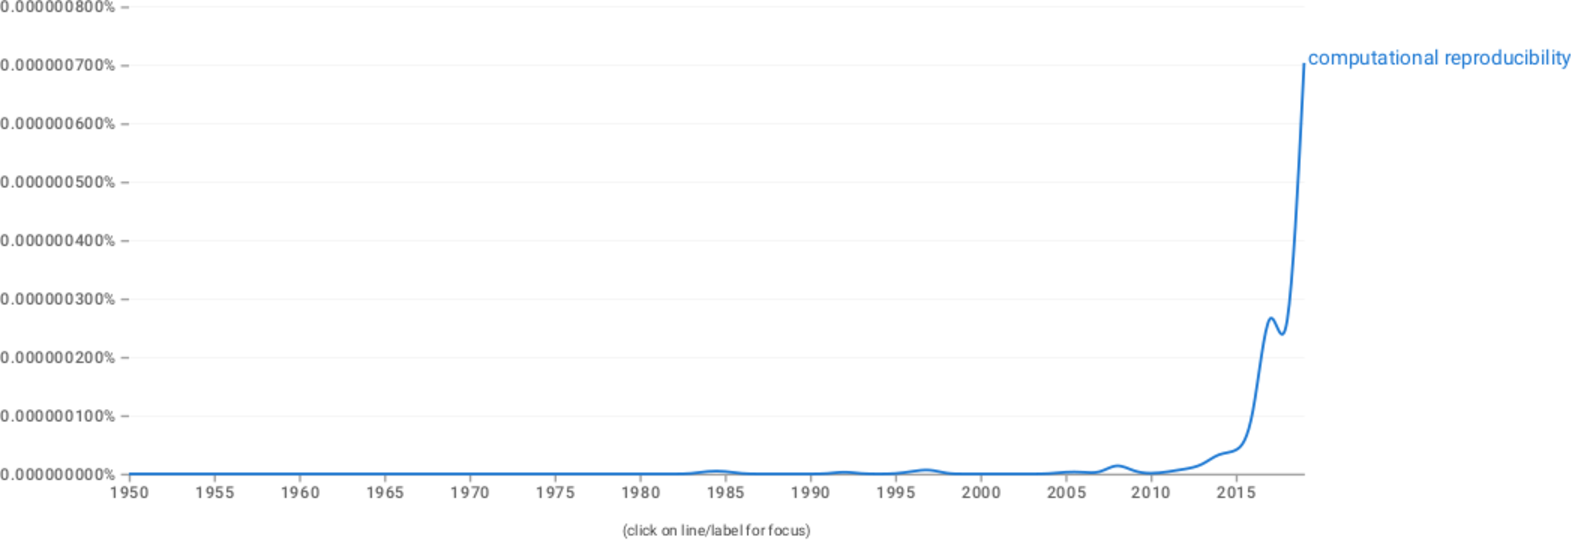
\includegraphics[width=\textwidth]{google_ngram_reproducibility_2023-05-08.pdf}
	\caption[Computational reproducibility in the literature]{Popularity of computational reproducibility: A chart of the frequencies of the n-gram ``computational reproducibility" (using yearly count, normalized be the numbers of publications in each year) in literature included in the English(2019) corpus of Google books. This graph has been created using the Google Ngram Viewer (\href{https://books.google.com/ngrams/info}{books.google.com/ngrams}) \citep{michel2011quantitative}}
	\label{fig:ngram}
\end{figure}


\subsection{``Everything matters'' for computational reproducibility in neuroimaging}

% maybe NARPS paper?`

The building blocks of research output extend to more than the files that constitute the actual research output, but also to all elements involved in its generation \citep{claerbout1992electronic}.
Consider different types of research output:
Raw data originates from acquisitions based on - potentially ongoing - experiments, raw data transformations, or data cleaning.
Processed data or results stem from computations with analysis code or software in specific versions on particular data.
And software, expressed in raw (code) or derived (transformed into executable) form, is created or used in specific computational environments, with compilers, underlying libraries, and systems in distinct versions.
Consequently, these building blocks play an integral part in the genesis of research outputs, and changes in these building blocks or their composition can translate to changes in the resulting research output.\\
Because of their complexity, neuroimaging studies face obstacles for reproducibility.
For one, the details of how code, software, or data have been used to generate a research output, such as analysis parameterization, the subset of data used as input, or sequence and invocation of employed software tools, are volatile.
Shared code and data does not always suffice to reproduce a result:
A study of data availability, reusability, and reproducibility demonstrated that well-described, ``in principle reusable'' data often does not suffice to reproduce the scientific findings of the corresponding publications due to  missing process provenance metadata \citep{hardwicke2018data}.
Secondly, even if methods and their sequence are well-described, precise information about the employed software tools is crucial, too.
The fact that different neuroimaging analysis software can produce distinct results from the same data despite using similar conceptual methodology is well known \citep{bowring2019exploring}.
This has been attributed to implementation differences \citep{palumbo2019evaluation}, software errors \citep{eklund2016cluster}, or analytic configurations \citep{pauli2016exploring}.
For example, in task-based fMRI, \citet{li2021moving} found that the choice of output space or resolution can have a marked impact on variability between conceptually similar processing pipelines.
Moreover, even with identical pipelines and data, surprising result variability can occur with minor variations in parametrization.
\citet{mueller2017commentary} reported that the choice of resampling resolution impacts alpha inflation, and \citet{li2021moving} identified the decision whether or not to include global signal regression as a major source of intra-pipeline variation.
Finally, even the same analysis, with identical parametrization, software tool, and data, can result in different outcomes if it is repeated across different operating systems, or with differences in versions of a singular software tool or operating system \citep{gronenschild2012effects, glatard2015reproducibility}.
%more here
Computational reproducibility across computing environments thus often remains elusive unless accounted for from the very start.
Therefore, in addition to ``Everything matters'',  \citet{kennedy2019everything} cued the phrase ``Reproducible by Design (as opposed to reproducibility as an afterthought)'' for conducting research in a way that makes computational reproducibility possible.
The next section highlights a number of strategies for this.

% However, a growing number of studies suggest that differences in the implementation of these processing steps or how they are “glued together” can yield notably different outcomes. Studies systematically comparing specific preprocessing steps such as segmentation15, motion correction16, and registration17–19 have reported substantial variation in outputs generated across independently developed packages when applied to the same data. In the analysis of task fMRI data, end-to-end pipelines built using different software packages have been found to produce marked variation in the final results20–23. from https://www.biorxiv.org/content/10.1101/2021.12.01.470790v2.full


\section{Towards re-usable research objects}


The reusability of research objects has become a distinct characteristic of scientific practice as it allows for reproduction, verification, building up upon and extending existing work, evidence synthesis, and minimizing duplicate efforts in the advancement of science \citep{thanos2017research}.
With this, it maximizes the impact of the funding and work that resulted in the research output.
Therefore, it is considered the “ultimate goal” of the FAIR principles \citep{wilkinson2016fair}, and an explicit and central expectation in a variety of funding sources such as the Economic and Social Research Council (ESRC, UK), the European Research Council (ERC, EU), or the National Institutes of Health (NIH, US).
In the scope of the FAIR principles, reusability focuses on the ability of a human or a machine to decide if data are useful and usable in a particular context based on richly curated metadata.
This reusability requires trust \citep{bechhofer2010research}. Re-users must be able to audit the steps performed in an experiment or analysis in order to be convinced of the validity of the results or derivatives.
FAIR principle R1.2, ``(Meta)data are associated with detailed provenance'' \citep{wilkinson2016fair}, refers to this.
This principles also encodes the process provenance necessary for reproducibility.
And indeed, reproducibility and trust are closely related:
Where resources are not fully FAIR yet, manual reproducibility typically provides the trust that process provenance would otherwise provide.
A new project, for example, typically starts with a check if the previous foundational findings still hold.\\
Many scientific fields or projects argue that FAIRness requires coordinated use of ontologies for metadata and brought forward efforts for ontology development and consensus building \citep[e.g.,][]{wise2019implementation, abrams2022standards, papadiamantis2020metadata}, but not in all domains are the necessary metadata standards incentivized or ready to use.
A few years before the publication of the FAIR principles, \citet{bechhofer2013linked} cued the term ``reusable research object'' in a conceptual position paper, and defined it as a ``container for a principled aggregation of resources, produced and consumed by common services and shareable within and across organisational boundaries. [...It] includes not only the data used, and methods employed to produce and analyse that data, but also the people involved in the investigation. An association with a dataset (or service, or result collection, or instrument) is now more than just a citation or reference to that dataset (or service or result collection). The association is rather a link to that dataset (or service or result collection) that can be explicitly followed or dereferenced providing access to the actual resource and thus enactment of the service, query or retrieval of data, and so on.''
% Detail how datalad adheres to these requirements.
In the following, I will highlight four properties that DataLad dataset or its contents possess that make them a reusable research object \citep{wagnerohbm2021}: Versioned, actionable, modular, and portable.
% and argue why the \gls{rdm} features that DataLad provides assist with FAIRification.

\subsubsection{Versioned}

The information ``I generated X from data Y with software Z'' is insufficient for reproducibility and trustworthiness if Y exists in multiple versions or subsets, if different releases of Z have relevant implementation differences, or if Z behaves differently depending on the environment it is used in.
If digital research objects are exhaustively tracked, they can be accessed and used transparently in a uniquely identified version state.
This exhaustive identity registration removes ambiguity that arises if the files in question are not completely static.
Therefore, the first relevant feature that DataLad provides for reproducibility is version control for all relevant files -- from data to code to software environments.
It lays the foundation for exhaustive tracking, and the DataLad dataset is a suitable overlay structure to include every relevant element for a scientific project.

\subsubsection{Actionable}

Process provenance metadata how a file came to be is often incomplete and difficult to retrace \citep{hardwicke2018data}.
It is tedious, often without an immediate benefit for curators, and rarely explicitly incentivized to retrospectively annotate research objects with process provenance \citep{edwards2011science, san2009long}.
Rather, this information should be captured at the time of creation, with the tools and persons that are involved in the creation of research outputs anyway \citep{dallas2016digital}.
But while early curation can increase the comprehensiveness of metadata, additional measures should guarantee its validity, as even fully described research outputs fail to be reproducible or reusable if their description or provenance contains errors \citep[see, e.g.,][]{manninen2017reproducibility}.
The most pragmatic approach to valid metadata is to base subsequent processing on them.
In the simplest case, this can be a codified parametrization of an analysis in a configuration or analysis design file  \citep[see, e.g.,][]{jas2018reproducible}.
If an analysis based on it completes successfully, it constitutes valid provenance metadata, created by an expert or automatically at the earliest possible time at no additional cost, and adds immediate benefit for curators as it captures relevant provenance and detects erroneous or missing metadata in passing.
This process is easiest if the tools used during the creation of a research output use the same metadata that gets eventually published alongside the final research output.
Therefore, a second relevant feature is actionable metadata.
Even if this metadata does not follow established community standards as required by the \gls{FAIR} principles yet, it preserves knowledge that would otherwise be lost, without requiring additional training, impeding later additions, or putting additional burden on scientists - it is a byproduct of standard scientific practice.


\subsubsection{Modular}

The reusability of scientific work can improve if it is accessible in modular units that constitute unambiguous multi-use components, such as raw data, processed data, or software.
In the simplest case, modularization means placing conceptually distinct content into separate files, and grouping files in individual directories to reflect more global structures.
Distinct units, such as the directories ``code/'' and ``inputs/'', increase transparency if each location is associated with distinguishable content, ease flexible recombination of such components into new projects, allow continuous evolution of an individual module without impact on other components of a project, and enable location-specific access control.
Thus, a third feature is modularity.
Though a single modular unit can not entail all relevant elements of a scientific study or data analysis, exhaustive tracking of all elements without sacrificing modularity can be achieved by linking multiple modular units in dependency relationships.
A useful metaphor are package management systems such as conda (\url{https://docs.conda.io}) or APT (\url{https://wiki.debian.org/Apt}): A software package is a modular unit, installed with a package manager.
However, packages usually depend on other software packages, which are listed as its ``dependencies''.
During installation, package managers check if all of the linked dependencies exist on the system, and if not, install them in the required versions automatically.
In scientific projects, modular units (data, software, code) are the dependencies of a given research output.
When those units are tracked, dependency relationships can include precise versions.
Beyond transparency and tidiness, modularization and linkage thus provide methods for reuse with which stand-alone units can be assembled into new projects, and research output contains the pieces it was derived from as linked dependencies \citep{bechhofer2010research}.


\subsubsection{Portable}

The fourth property is portability.
The more portable a digital research object is, the easier it is to reuse it.
A research object is fully portable if no adjustments are necessary for it to function the way it is intended to on different computational infrastructure -- ideally even when used by a naive re-user with a different area of expertise (i.e., without domain knowledge).
The more adjustment or domain knowledge is necessary, the less portable a research output becomes.
A factor contributing to portability self-containment such that research outputs can be used or reproduced on different computational infrastructure by other users.
Completeness is crucial for this, and a research output should be accompanied by the necessary code, data, and computational environment to produce it.
Self-containment also entails that a project can be moved across computers and remains functional without adjustment, for example by ensuring that no references to file system, operating system, or user specific idiosyncrasies are included.
Only if a re-user does not need to modify project files, they can be certain that they did not inadvertently break or influence the output with it.

\begin{figure}
	\centering
	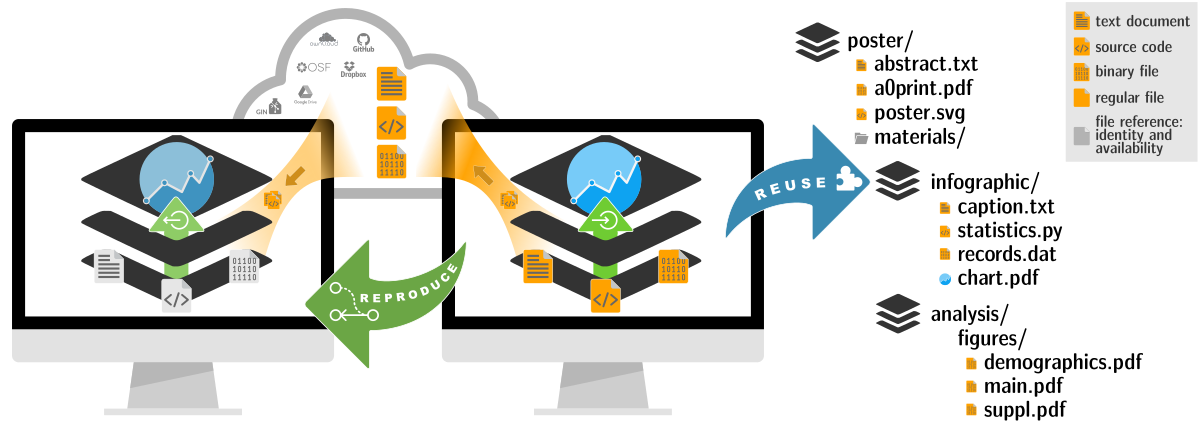
\includegraphics[width=.9\textwidth]{vamp.png}
	\caption[DataLad datasets as reusable research objects]{Reusing research outputs implies trust, and trust should be earned through verification. Verification is enabled by provenance information. Provenance capture of research outcomes requires exhaustive tracking of all inputs, as well as process records that describe how inputs were combined and transformed to generate outputs (middle). When lightweight metadata are actionable, they can be used to reproduce research outputs in a different environment from precisely identified inputs by (re-)applying the recorded process (left). A data structure that affords this type of portable recomputation is a self-contained unit that can be reused as a modular input component for incremental research (right).
	}
	\label{fig:vamp}
\end{figure}




% curation needs to be pragmatic

Although FAIR research objects are universally desirable, in practice, the necessary standards and procedures for creating FAIR (meta)data are not always already in place when research is conducted.
This can turn FAIRification into a bureaucratic data governance effort, diminishing the immediately obvious benefits for the curator \citep{zehl2016handling}.
However, the four properties outlined above are a big step into the right direction, and essentially a byproduct from pragmatic research data management in DataLad datasets.
\cref{fig:vamp} illustrates how it yields trusted and reusable research objects, and the next section details a technical implementation and proof-of-concept analysis to create such reusable research objects as a byproduct of \gls{rdm} in analyses of any scale.

\pagebreak

\section{FAIRly big: A framework for computationally reproducible processing of large-scale data}

% role of sample size for reproducible results: \citep{li2021moving}

%  \citep{li2021moving} "highlight the reality that as the test-retest reliability approaches optimal levels for laboratory measurement, pipeline implementation differences will impose an inherent upper bound on the agreement of preprocessed data. These findings also underscore that 10 minutes of data, which has been common in the field until at least recent years, are insufficient for producing results that are reliable enough to reveal substantive pipeline-related variation."

\begin{figure}
	\centering
	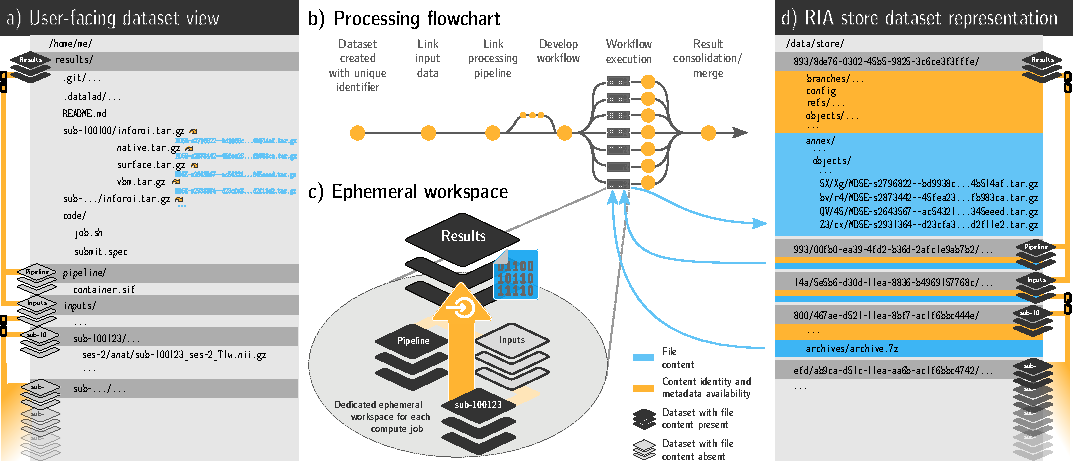
\includegraphics[width=\textwidth]{ukbworkflow_simplified.pdf}
	\caption[]{}
	\label{fig:fairly_workflow}
\end{figure}

\begin{figure}
	\centering
	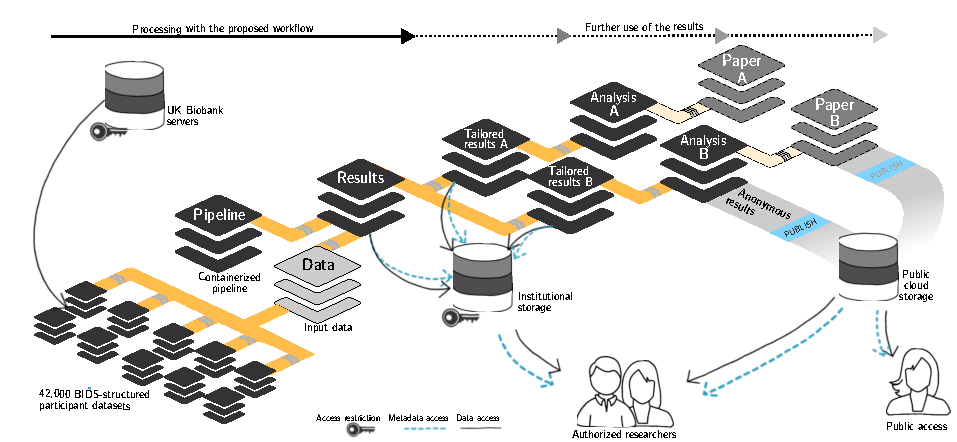
\includegraphics[width=\textwidth]{ukb_datasets.pdf}
	\caption[]{}
	\label{fig:fairly_datasets}
\end{figure}

\begin{figure}
	\centering
	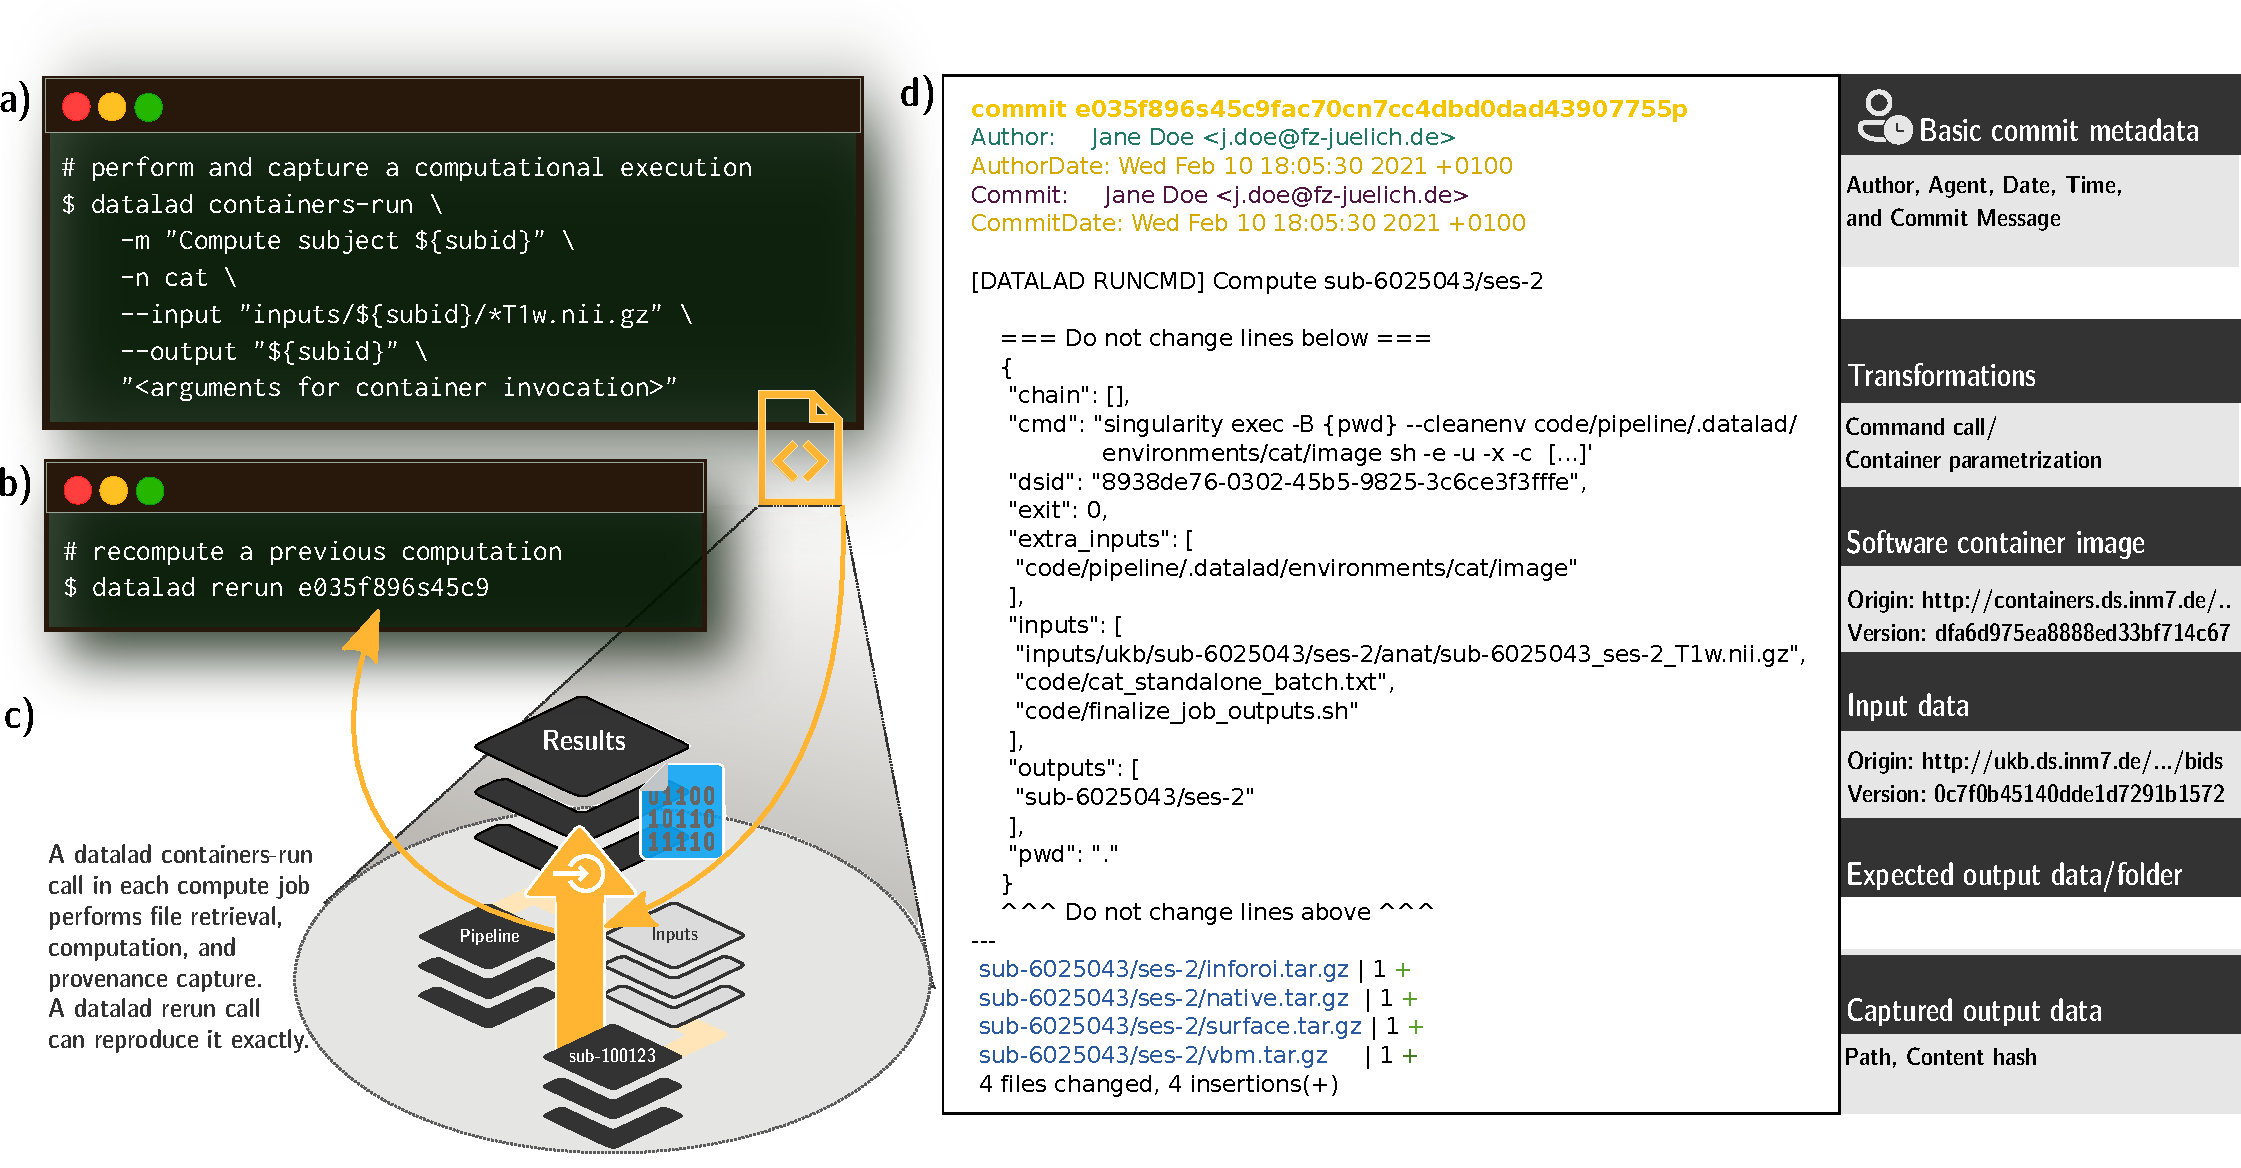
\includegraphics[width=\textwidth]{coarsemetadata.pdf}
	\caption[]{}
	\label{fig:fairly_metadata}
\end{figure}

% on re-analyzing the pipeline, cite li2021moving: "we demonstrated the role that pipeline replication can play as a means of exploring analytic variation and assessing the robustness of findings. To this end, we leveraged and extended the flexibility of C-PAC to replicate non-MATLAB dependent minimal processing pipelines (ABCD-BIDS, CCS, fMRIPrep-LTS) in a single platform"


\pagebreak